\documentclass[runningheads]{llncs}
%
\usepackage[T1]{fontenc}
\usepackage{graphicx}
\usepackage{booktabs}
\usepackage{xcolor}
\usepackage{hyperref}
\renewcommand\UrlFont{\color{blue}\rmfamily}
\urlstyle{rm}
%
\graphicspath{{../bench/results/}}
\newcommand{\plan}[1]{{\color{blue}\itshape[#1]}}
%
\begin{document}
%
\title{Accelerating Large-Scale Decision Tree Induction on Heterogeneous CPU-GPU Architectures}
\titlerunning{Decision Tree Induction on Heterogeneous CPU-GPU Architectures}
%
\author{Bruno Mirčevski\orcidID{0009-0007-1008-6708} \and
Krzysztof Jurczuk\orcidID{0000-0001-6469-1769}}
\authorrunning{B. Mirčevski and K. Jurczuk}
\institute{Faculty of Computer Science, Bialystok University of Technology,\\
Bialystok, Poland}
%
\maketitle
%

\begin{abstract}
We investigate parallel implementations of two widely used decision tree
induction algorithms, CART and C4.5, on multicore CPUs, CUDA-enabled GPUs, and
heterogeneous CPU-GPU architectures.

\keywords{Decision trees \and CART \and C4.5 \and Parallel computing}
\end{abstract}
%
%
\section{Introduction}
\label{sec:intro}

\section{Related Work}
\label{sec:related}

\subsection{Decision Tree Induction: CART and C4.5}
\plan{Brief: CART~\cite{breiman1984cart} (Gini, binary splits, cost-complexity
pruning), C4.5~\cite{quinlan1993c45} (gain ratio, MDL threshold cost,
error-based pruning). Only what is needed to read Sect.~\ref{sec:impl}.}

\subsection{Scalable and Parallel Induction on CPUs}

\subsection{Decision Trees on GPUs}

\section{Our Implementation and Optimizations}
\label{sec:impl}

\subsection{Simple}

\subsection{Serial}

\subsection{Parallel}

\subsection{GPU}

\subsection{Hybrid}

\section{Experiment Design}
\label{sec:design}

\subsection{Datasets}
\plan{One sentence per dataset (domain, how the test set is defined). All
features numeric; ECBDL's nominal features as integer codes. The GPUs train
ECBDL on its first 15M rows (80\,GB VRAM); SOREL does not fit on the GPUs.}

\begin{table}
\caption{Datasets. Sizes are of the training set as float32.}
\label{tab:datasets}
\centering
\small
\begin{tabular}{@{}lrrrrrl@{}}
\toprule
Dataset & Features & Classes & Training rows & Test rows & Size & Test set \\
\midrule
SUSY~\cite{baldi2014higgs}          & 18   & 2  & 4,500,000  & 500,000   & 0.3\,GB   & UCI split \\
HIGGS~\cite{baldi2014higgs}         & 28   & 2  & 10,500,000 & 500,000   & 1.2\,GB   & UCI split \\
ECBDL'14~\cite{triguero2015ecbdl}   & 631  & 2  & 31,992,921 & 2,897,917 & 80.8\,GB  & official \\
\quad GPU sample                    & 631  & 2  & 15,000,000 & 2,897,917 & 37.9\,GB  & official \\
MNIST8M~\cite{loosli2007mnist8m}    & 784  & 10 & 8,100,000  & 10,000    & 25.4\,GB  & MNIST test \\
SOREL-20M~\cite{harang2020sorel}    & 2381 & 2  & 12,699,013 & 4,195,042 & 120.9\,GB & official \\
\bottomrule
\end{tabular}
\end{table}

\subsection{Hardware}
\plan{Four nodes of the mordor3 cluster (Table~\ref{tab:hardware}), each used
whole (exclusive jobs). GPU nodes run the CUDA backend only, CPU nodes the CPU
backends and the other CPU implementations. GPU runs are bound to the GPU's
NUMA node (16 CPUs on hopper, 24 on ampere). Add measured memory bandwidth
(STREAM) per node. Software: Ubuntu 24.04, Linux 7.0, g++ 13.3 (\texttt{-O3}),
CUDA 12.9, NVIDIA driver 615.71.}

\begin{table}
\caption{Hardware. Every node has two sockets and no SMT; CPU, cores and L3
are per socket. One GPU (PCIe) is used per run.}
\label{tab:hardware}
\centering
\small
\begin{tabular}{@{}llrrrll@{}}
\toprule
Node & CPU (per socket) & Cores & Clock & L3 & RAM & GPU \\
\midrule
hopper & Xeon Gold 6444Y & 16 & 4.0\,GHz  & 45\,MB  & 1\,TB DDR5-4800   & H100 80\,GB \\
ampere & EPYC 7402       & 24 & 3.35\,GHz & 128\,MB & 1\,TB DDR4-3200   & A100 80\,GB \\
epyc1  & EPYC 9255       & 24 & 4.3\,GHz  & 128\,MB & 512\,GB DDR5-6400 & -- \\
dell1  & Xeon Gold 6542Y & 24 & 4.1\,GHz  & 60\,MB  & 1\,TB DDR5-5200   & -- \\
\bottomrule
\end{tabular}
\end{table}

\subsection{Compared Implementations}
\plan{./tree backends (\texttt{--simple}, \texttt{--serial},
\texttt{--parallel}, \texttt{--cuda}, \texttt{--gpu-only}); scikit-learn and
Weka J48 on the CPU; cuML and XGBoost on the GPU, with their settings. Why each
is the closest equivalent (no public GPU C4.5; J48 depth limit adapter;
XGBoost squared error = Gini on bins). rpart and YaDT: add or say why not.}

\subsection{Protocol and Measurement}
\plan{One tree, depth $\le$ 10, no pruning, all rows and features; what is
timed (training only, from data in memory; GPU setup and upload included);
peak RAM and VRAM; runs per case, means and spread; exclusive nodes; fairness
(CPU threads of the hybrid, warm library processes, input layout). Source:
docs/GPU-LIBRARIES.md, bench/README.md.}

\section{Results}
\label{sec:results}

\subsection{Comparison with Other CPU Implementations}
\plan{./tree's backends against scikit-learn (CART) and Weka J48 (C4.5):
time, memory, test accuracy, same trees.}

\begin{figure}
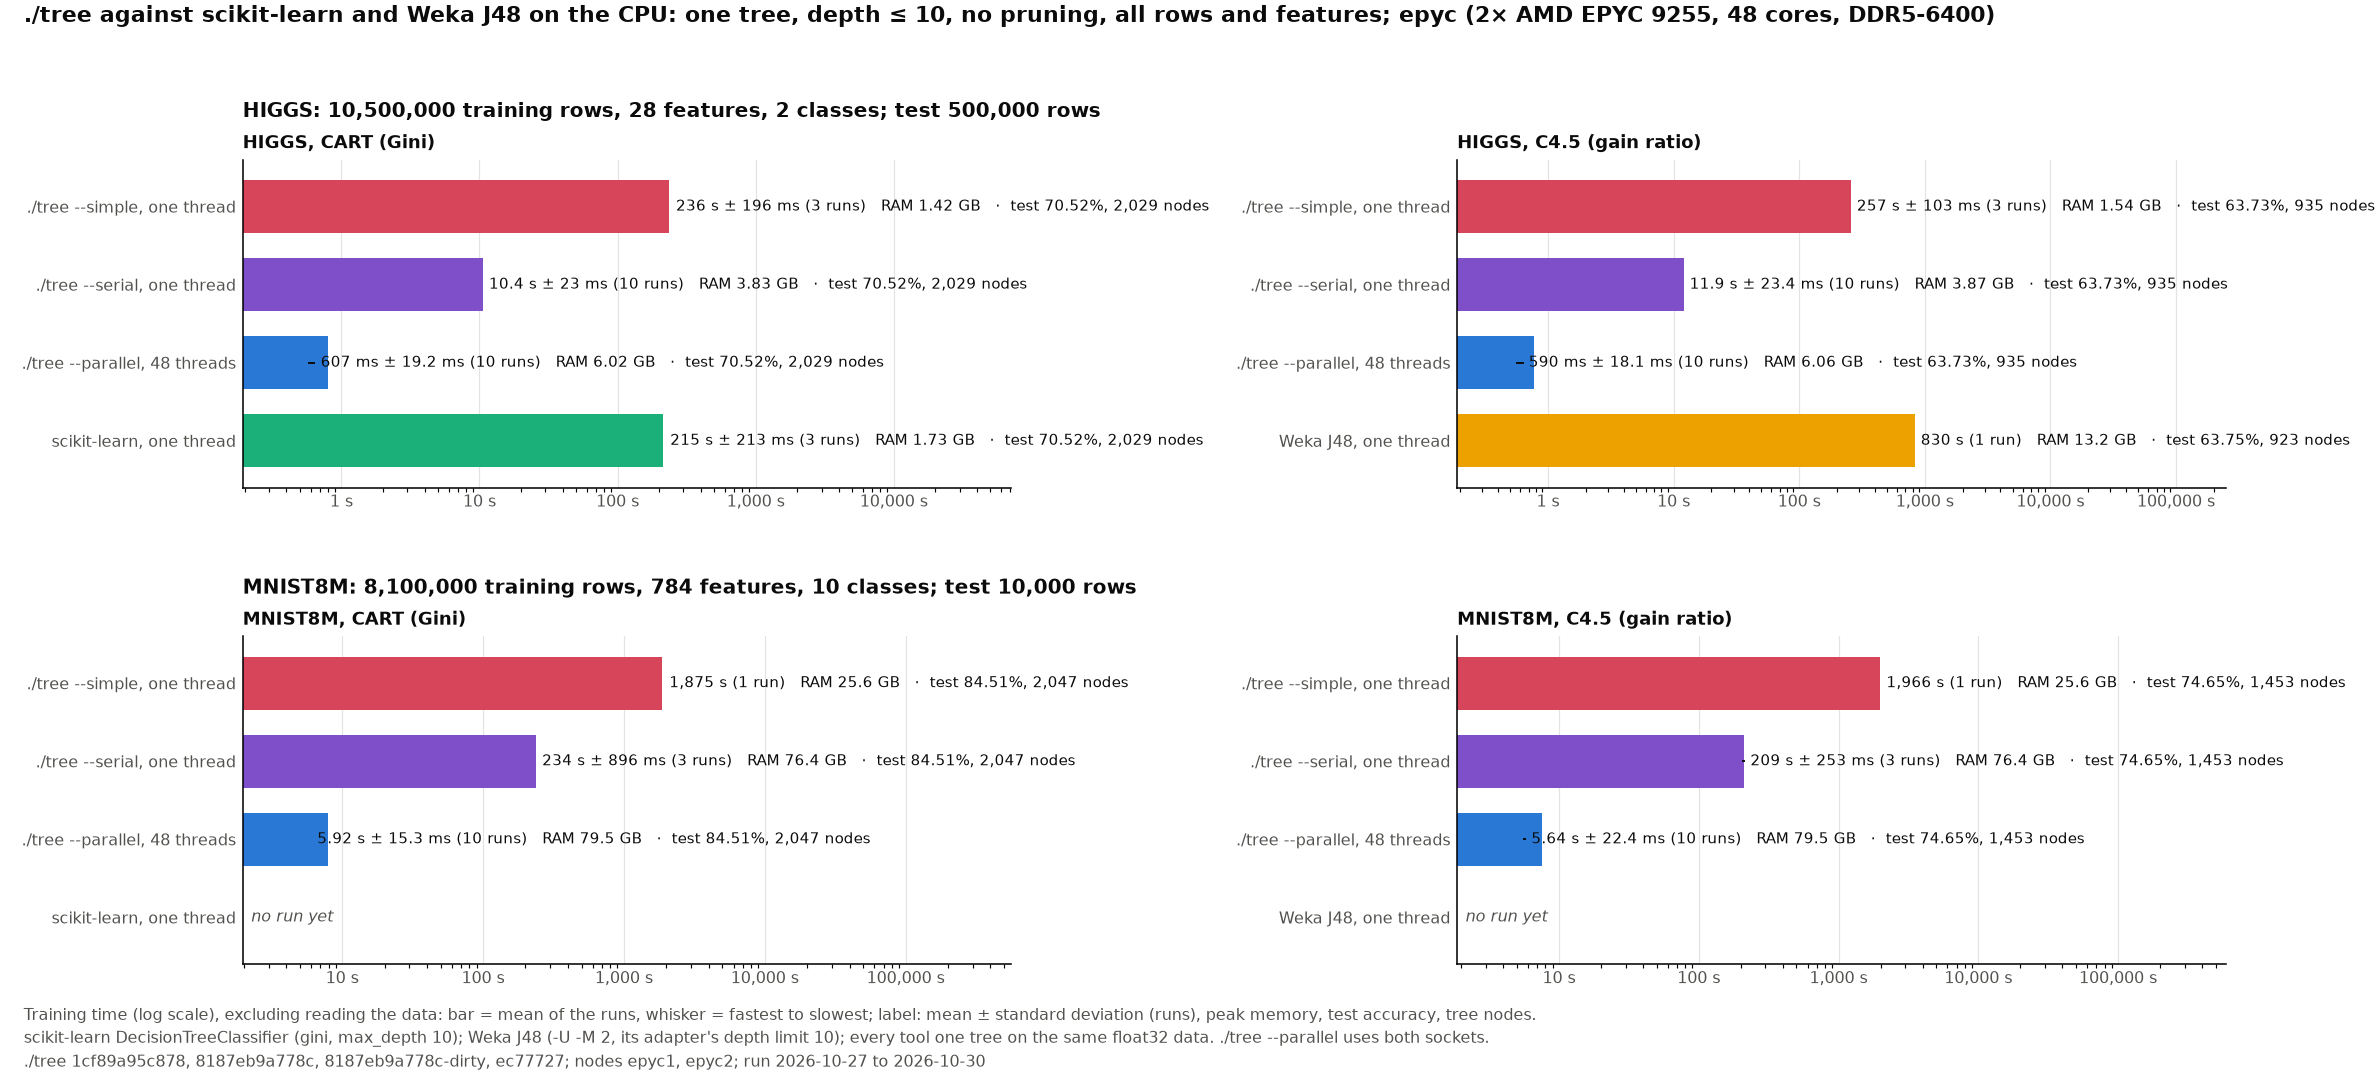
\includegraphics[width=\textwidth]{cluster-cpu-vs-others/chart.png}
\caption{Temporary: ./tree against scikit-learn and Weka J48 (cluster-cpu-vs-others).}
\label{fig:cpu-vs-others}
\end{figure}

\subsection{Comparison with GPU Libraries}
\plan{Against cuML and XGBoost: one tree, and per tree of a 10-tree forest;
accuracy of exact versus binned trees; VRAM.}

\begin{figure}
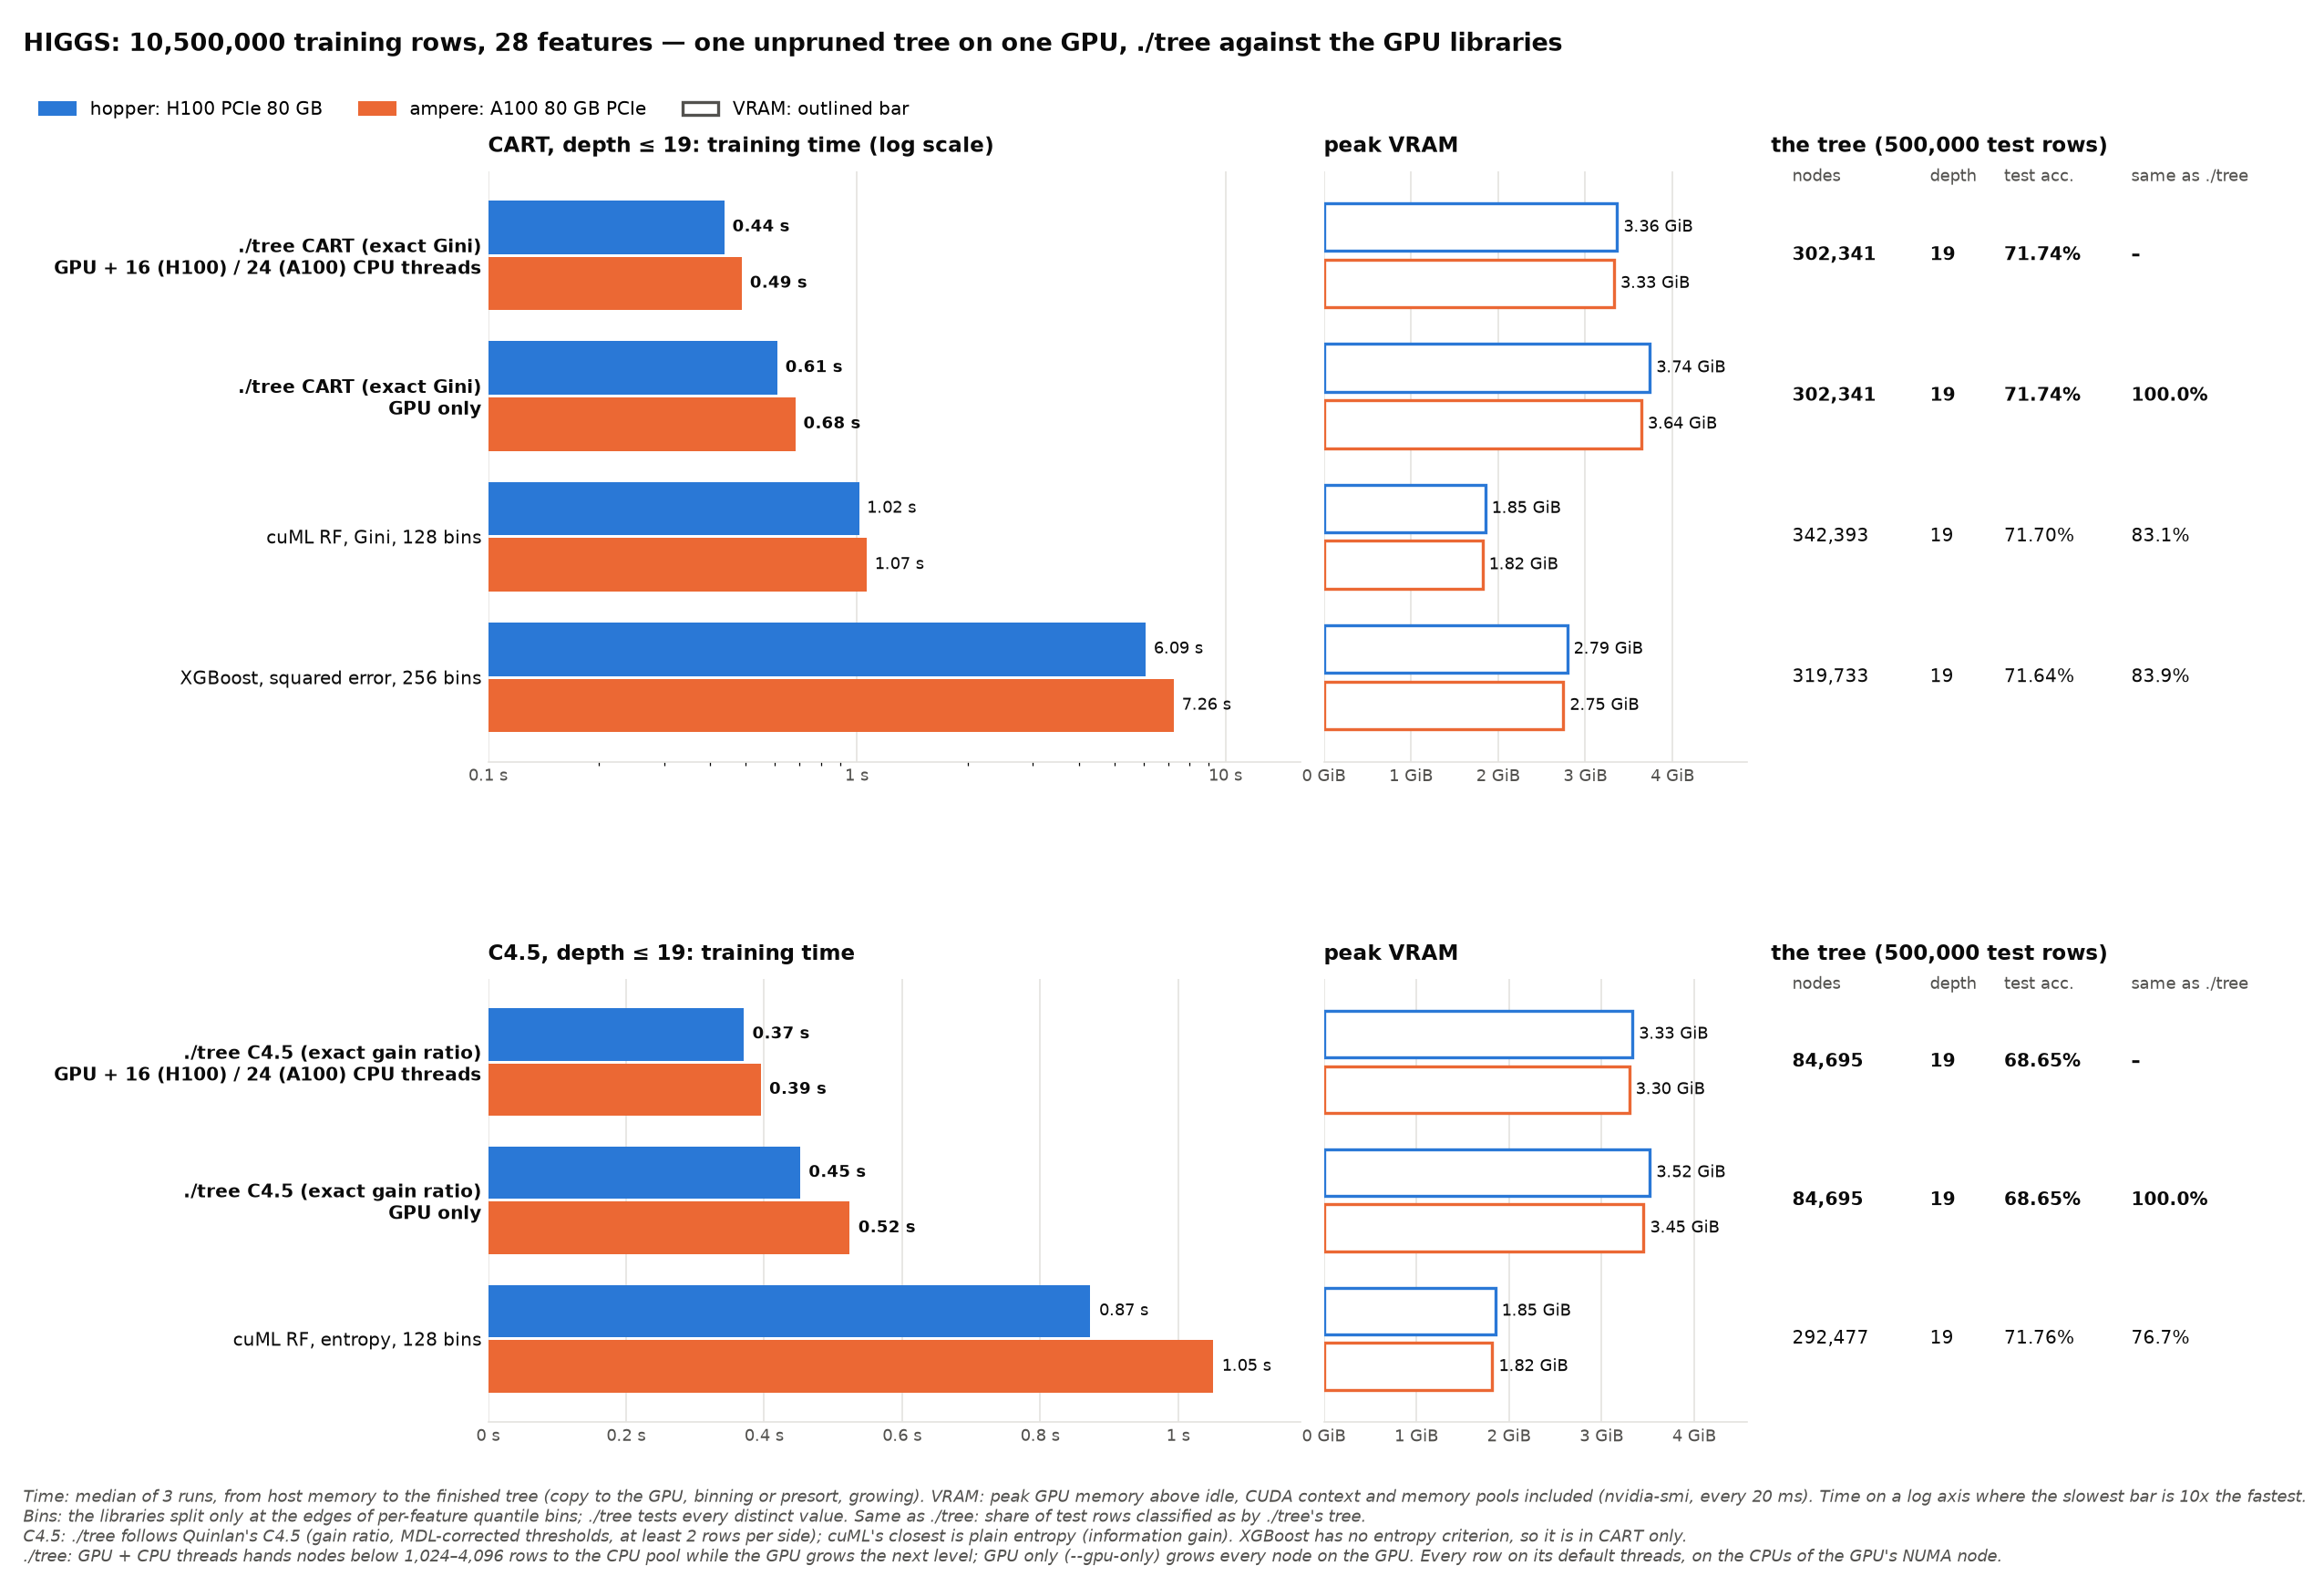
\includegraphics[width=0.49\textwidth]{cluster-gpu-vs-others/chart-higgs.png}\hfill
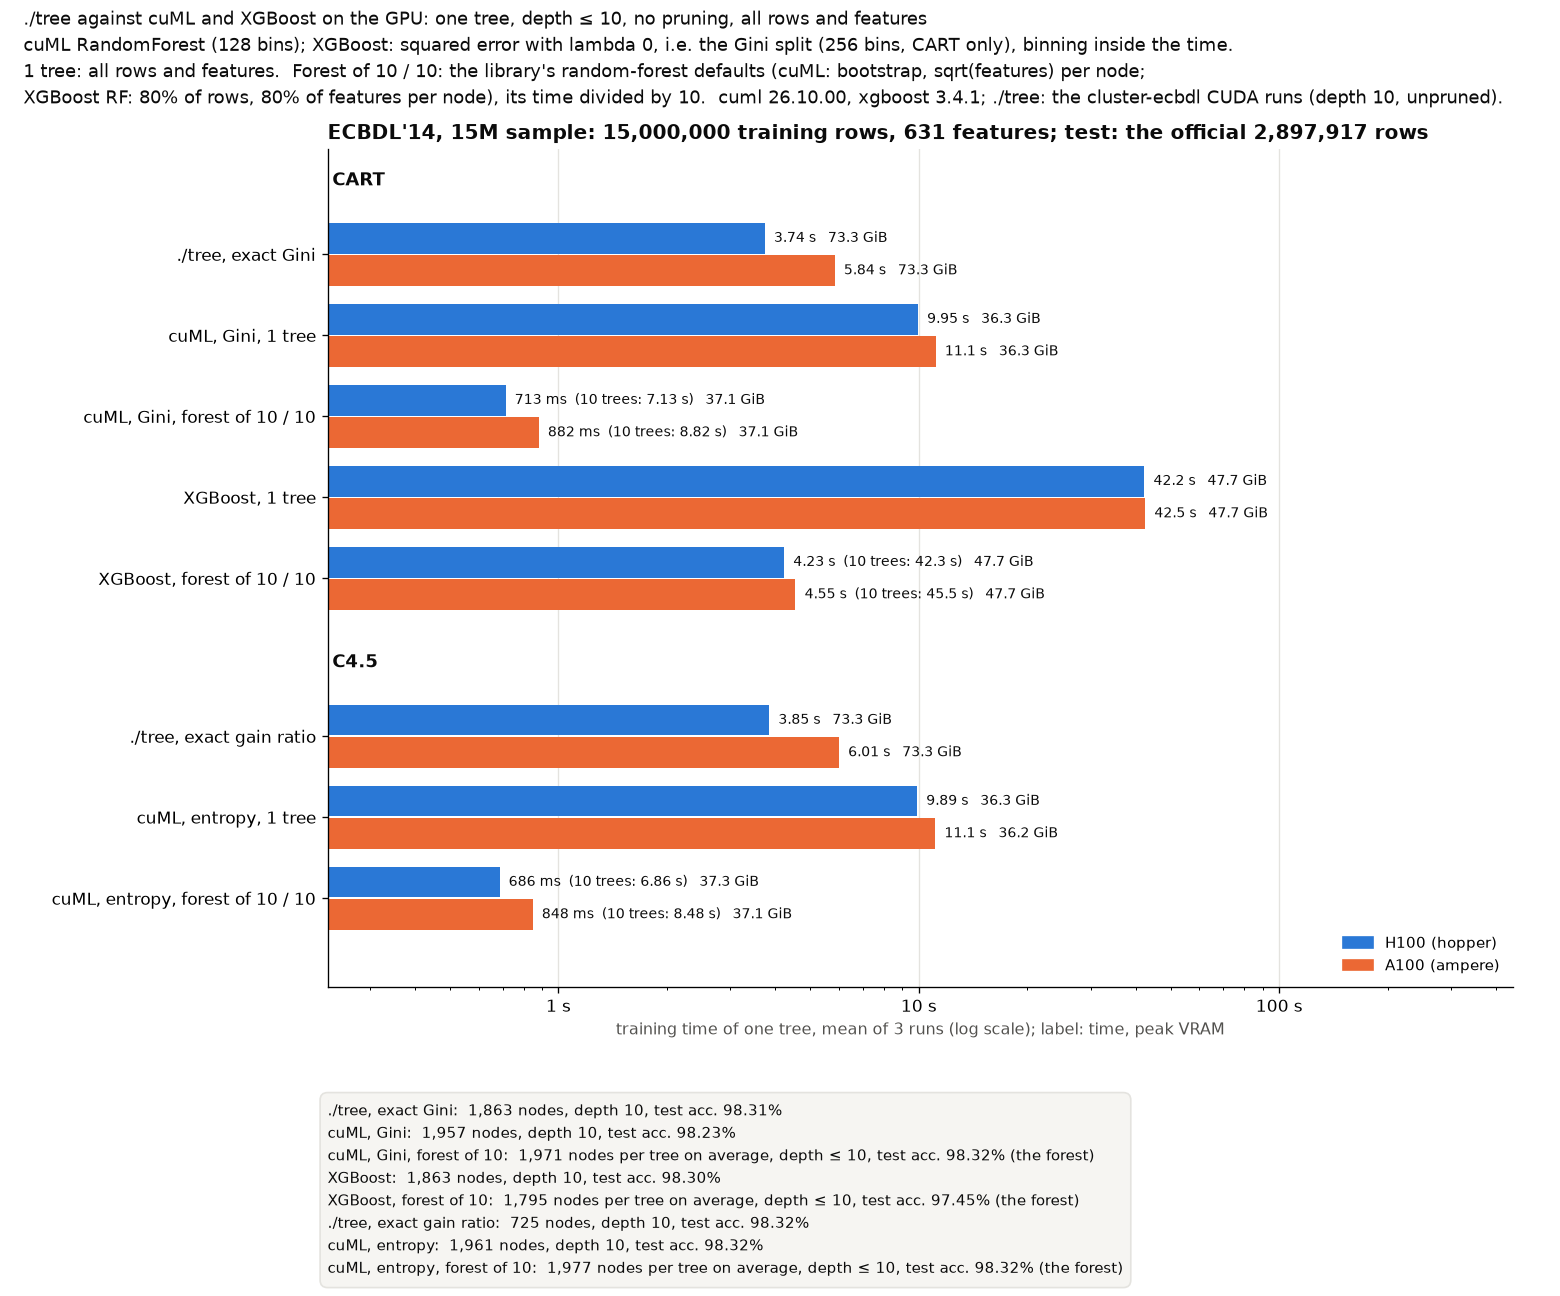
\includegraphics[width=0.49\textwidth]{cluster-gpu-vs-others/chart-ecbdl_15m.png}
\caption{Temporary: ./tree against cuML and XGBoost on HIGGS (left) and ECBDL'14 15M (right) (cluster-gpu-vs-others).}
\label{fig:gpu-vs-others}
\end{figure}

\subsection{Performance Across Hardware}
\plan{All ./tree backends on the four nodes, per dataset: serial, one and two
sockets, H100 and A100 hybrid and GPU only. CPU against GPU; which hardware
wins for which data shape (rows, features, classes).}

\begin{figure}
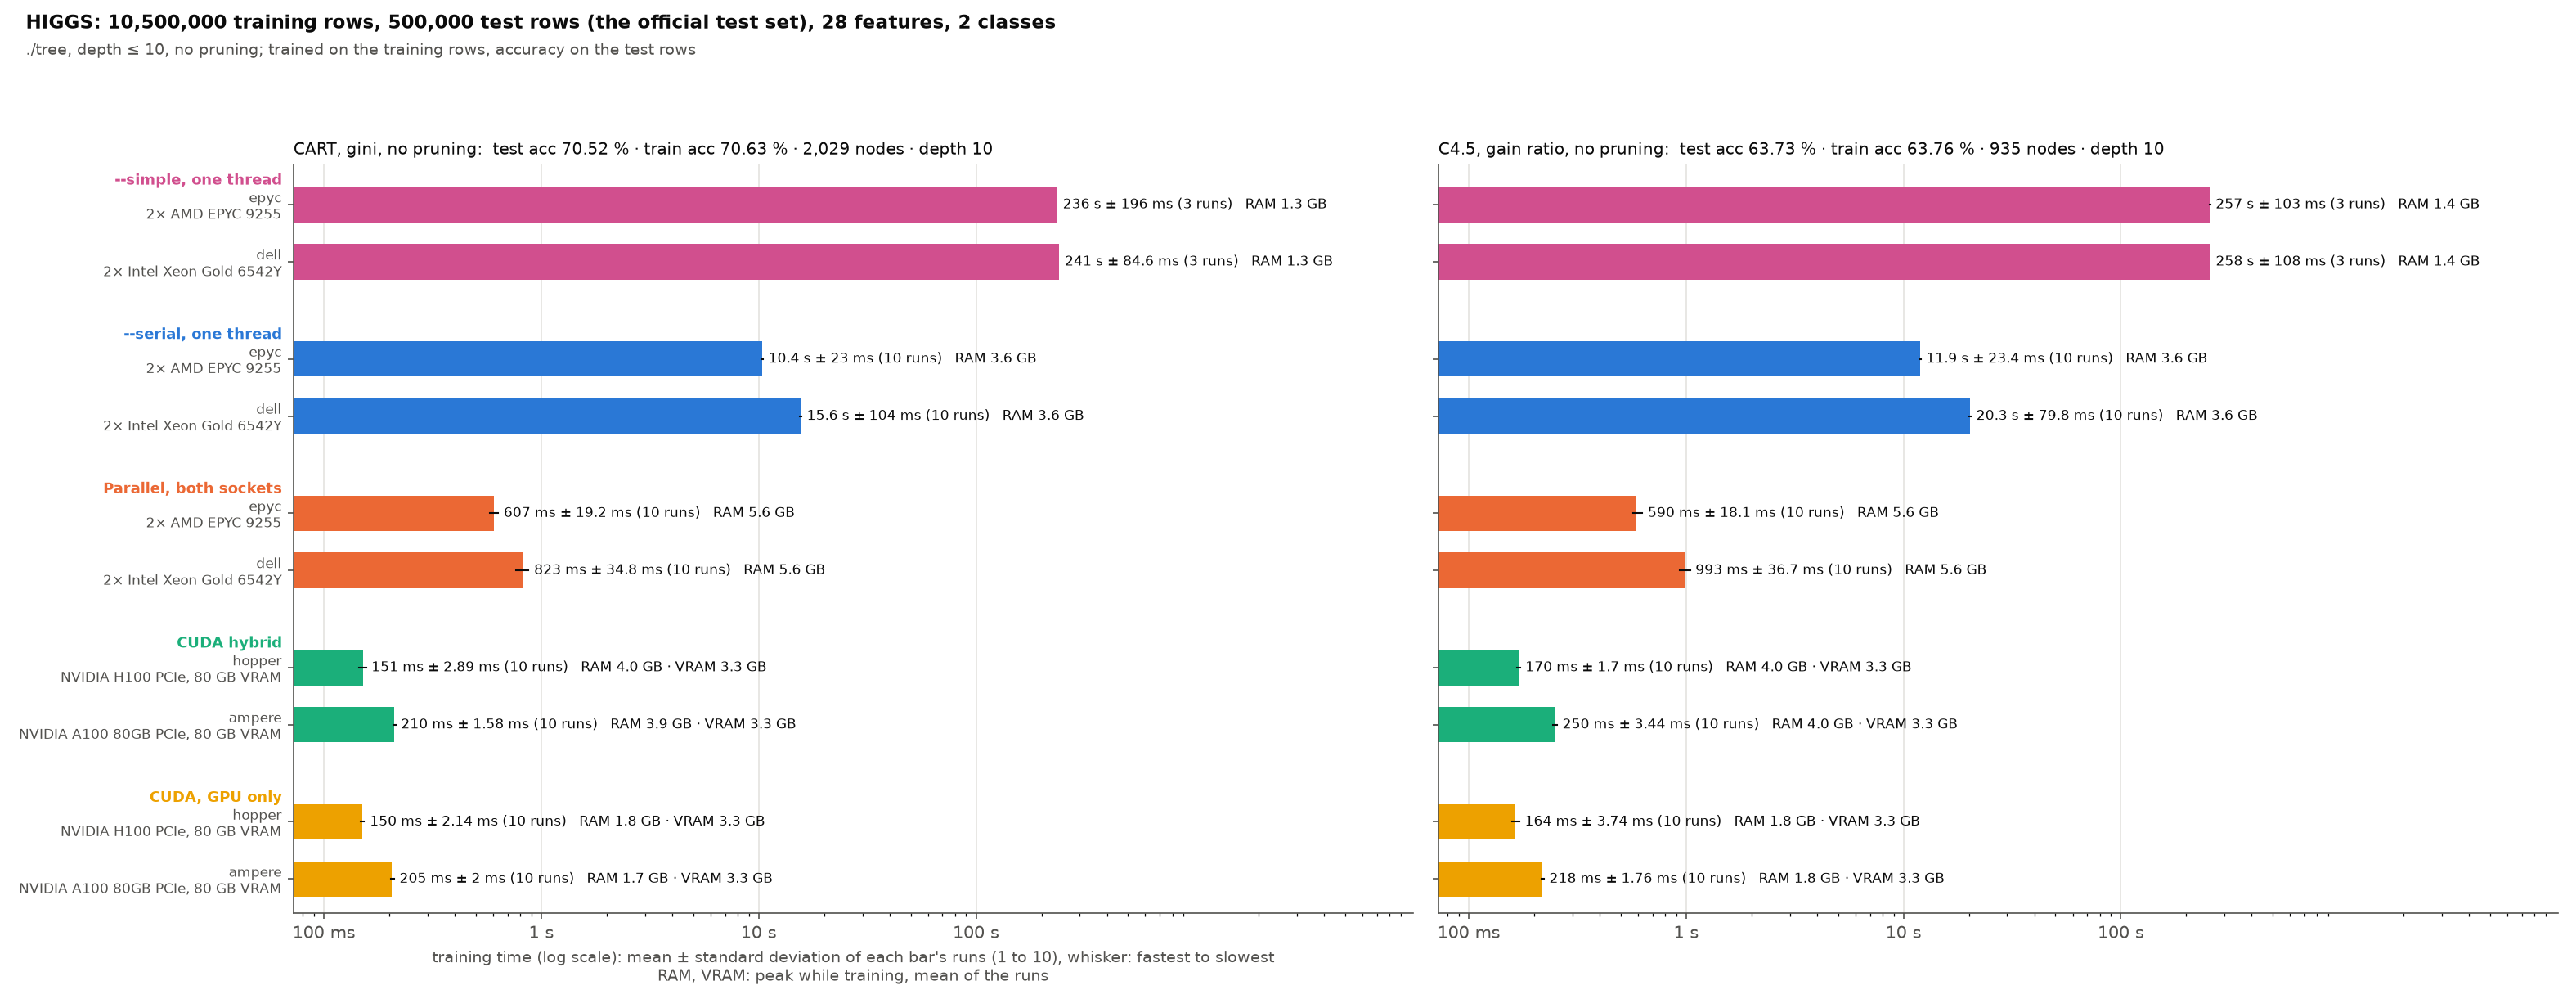
\includegraphics[width=\textwidth]{cluster-higgs/chart.png}
\caption{Temporary: ./tree's backends on HIGGS on every node (cluster-higgs).}
\label{fig:hardware-higgs}
\end{figure}

\subsection{Scalability}
\plan{Thread scaling 1--48 on epyc1 and dell1 (memory bandwidth bound); growth
with the number of rows (subsamples of one dataset).}

\begin{figure}
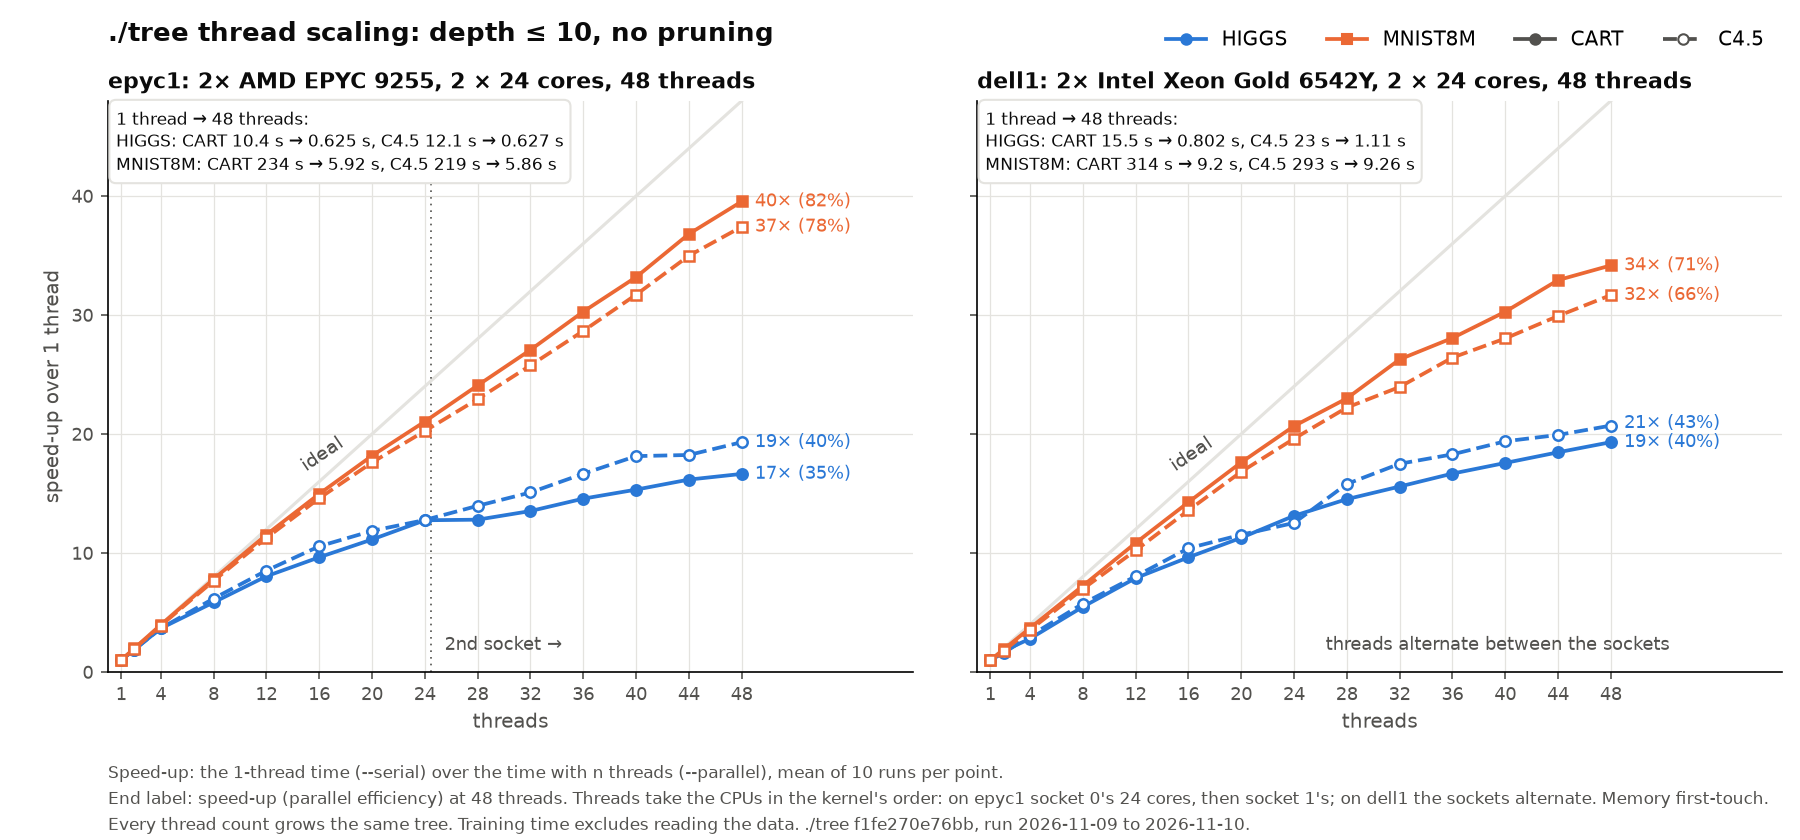
\includegraphics[width=\textwidth]{cluster-cpu-scaling/chart.png}
\caption{Temporary: thread scaling on HIGGS and MNIST8M (cluster-cpu-scaling).}
\label{fig:scaling}
\end{figure}

\subsection{Profiling}
\plan{Where the time goes: presort, split search, partition, CPU--GPU
transfer; GPU share of the hybrid; achieved bandwidth against peak.}

\begin{figure}
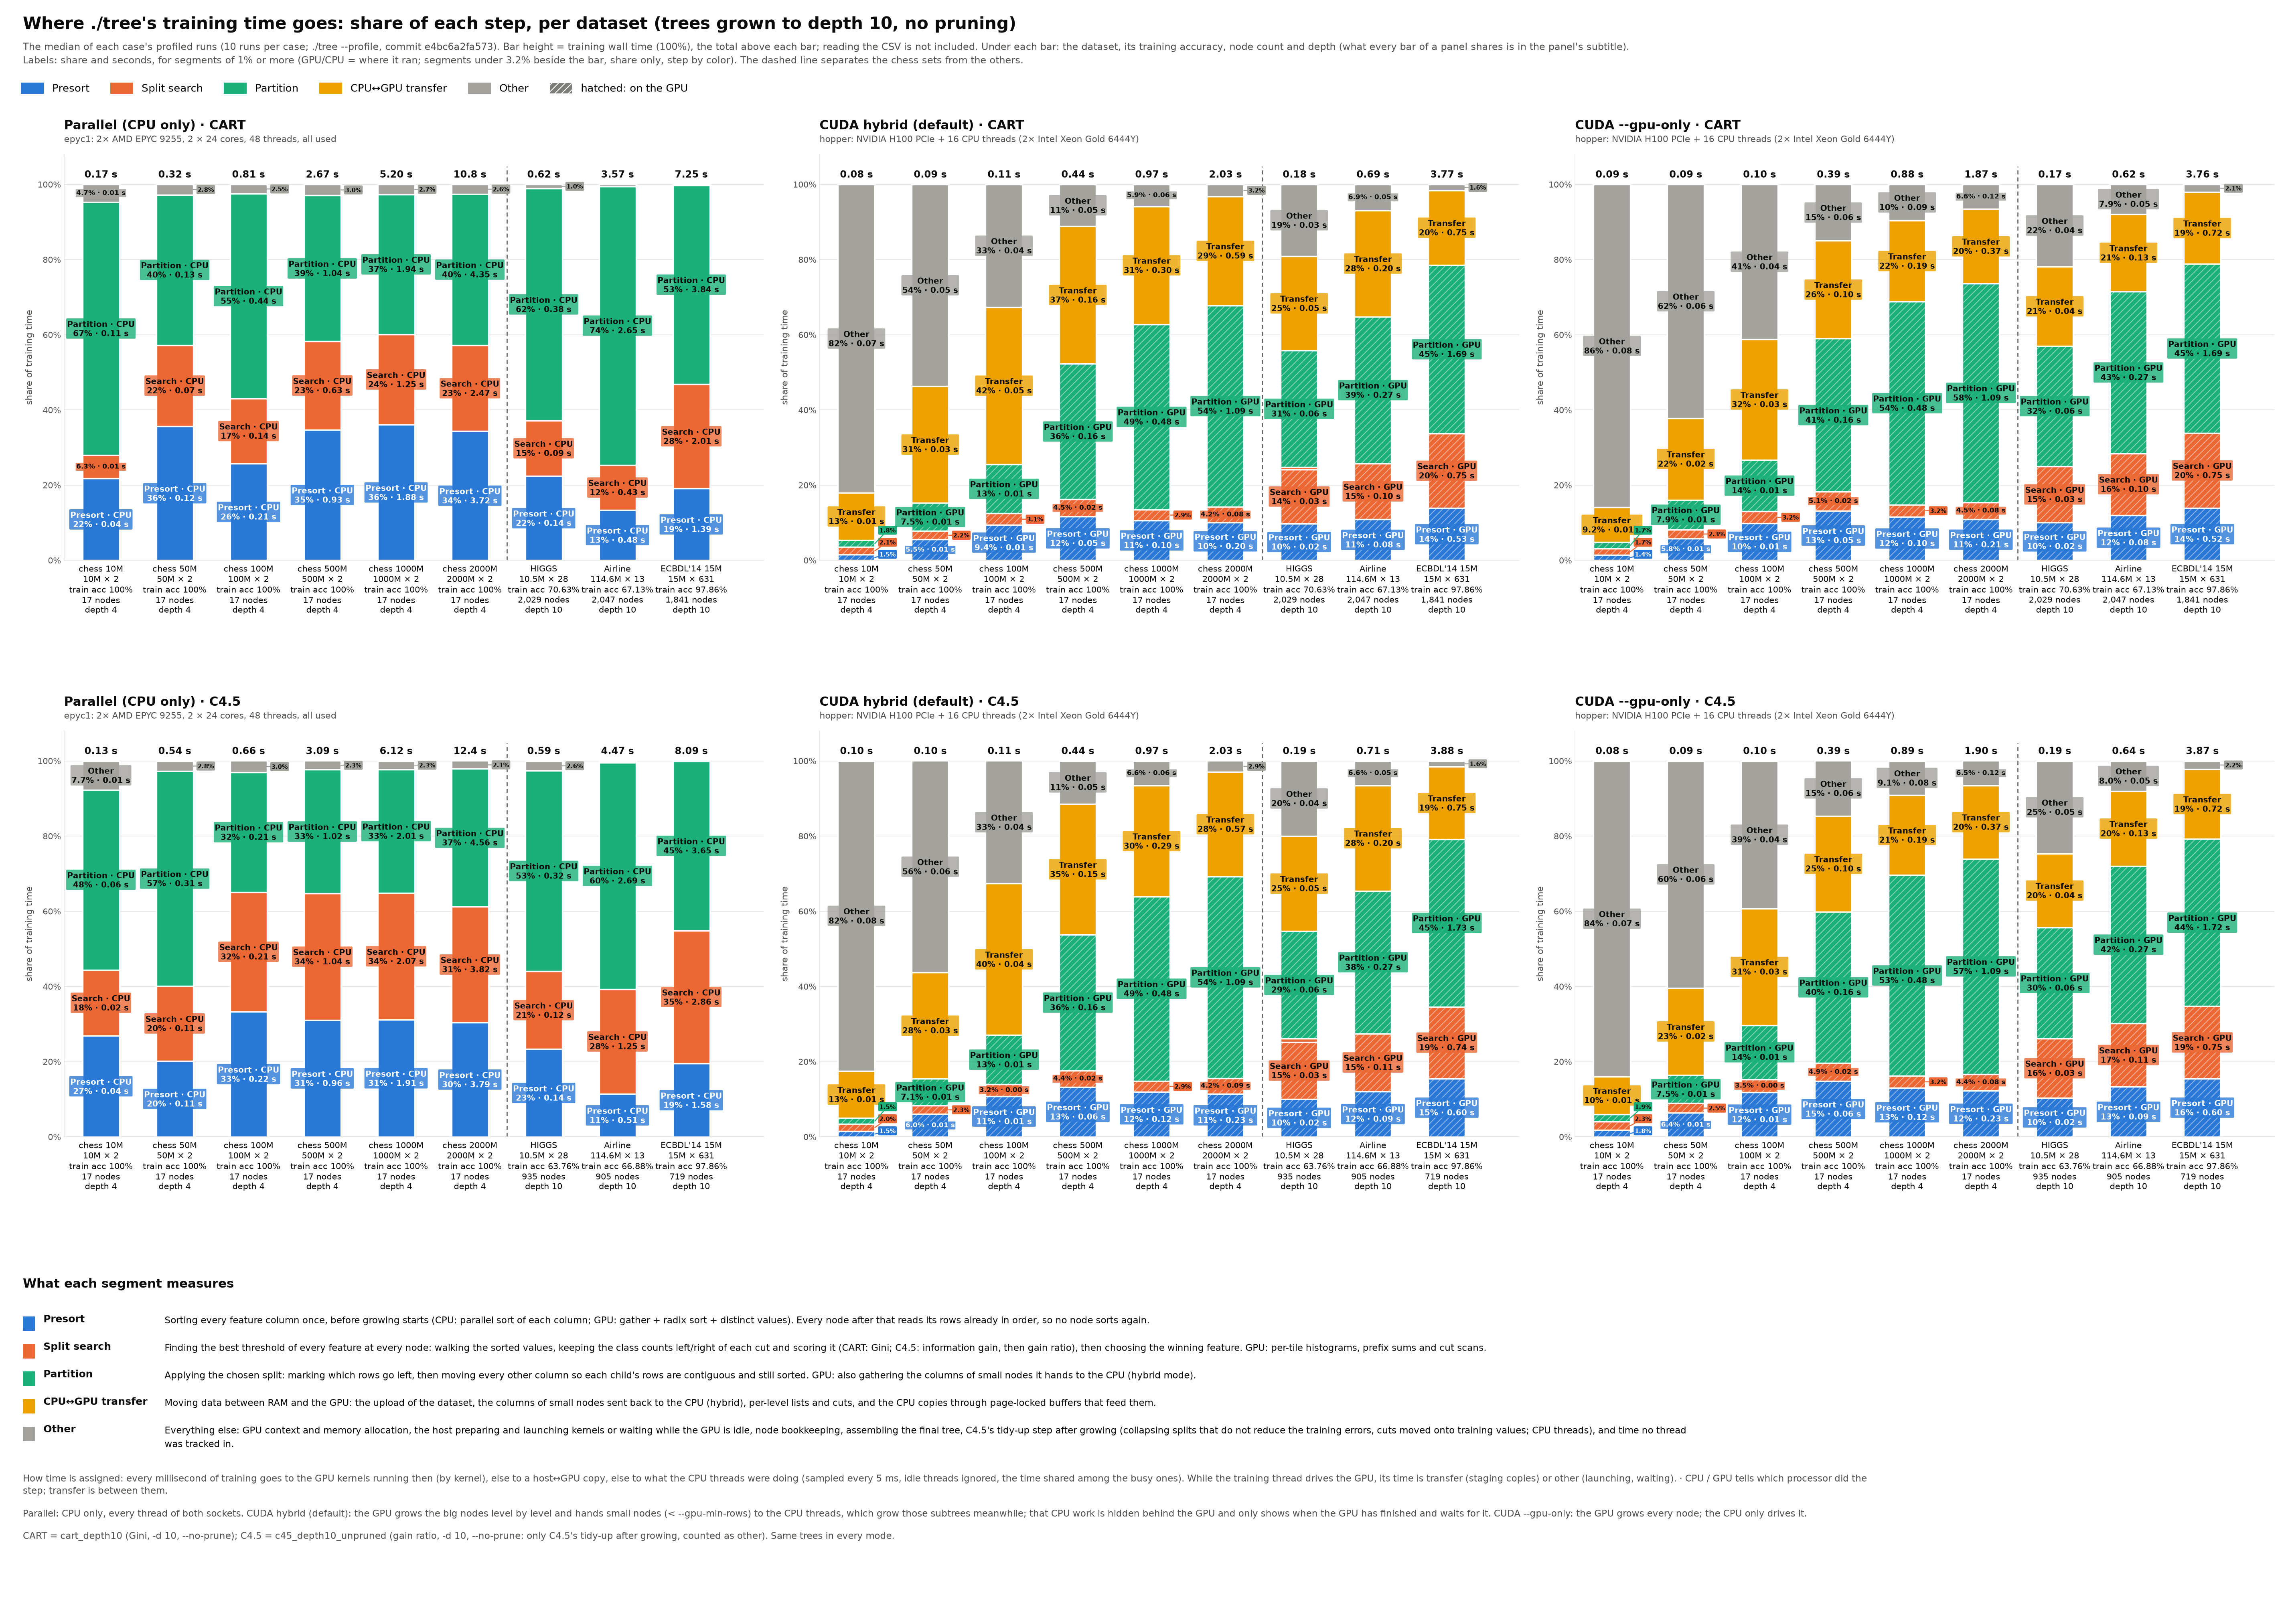
\includegraphics[width=\textwidth]{cluster-profiling/chart.png}
\caption{Temporary: breakdown of the growing time (cluster-profiling).}
\label{fig:profiling}
\end{figure}

\section{Discussion}
\label{sec:discussion}

\section{Conclusion}
\label{sec:conclusion}
\bibliographystyle{splncs04}
\bibliography{references}
%
\end{document}
